\chapter{Hypersonic Vehicle Model}

The Generic Hypersonic Vehicle which is used as a platform for analysis and control design is shown in Figure~\ref{fig.ghvclouds}.
The Road Runner GHV is a small, pilotless, blended wing-body vehicle, with 3-D inlet and nozzle, and axisymmetric through-flow scramjet engine.
There are four aerodynamic control surfaces which can be moved independently, consisting of two elevons and two rudders.
The relevant vehicle properties are listed in Table~\ref{tab:vehicle_properties}.

\begin{figure}[h]
  \begin{center}
    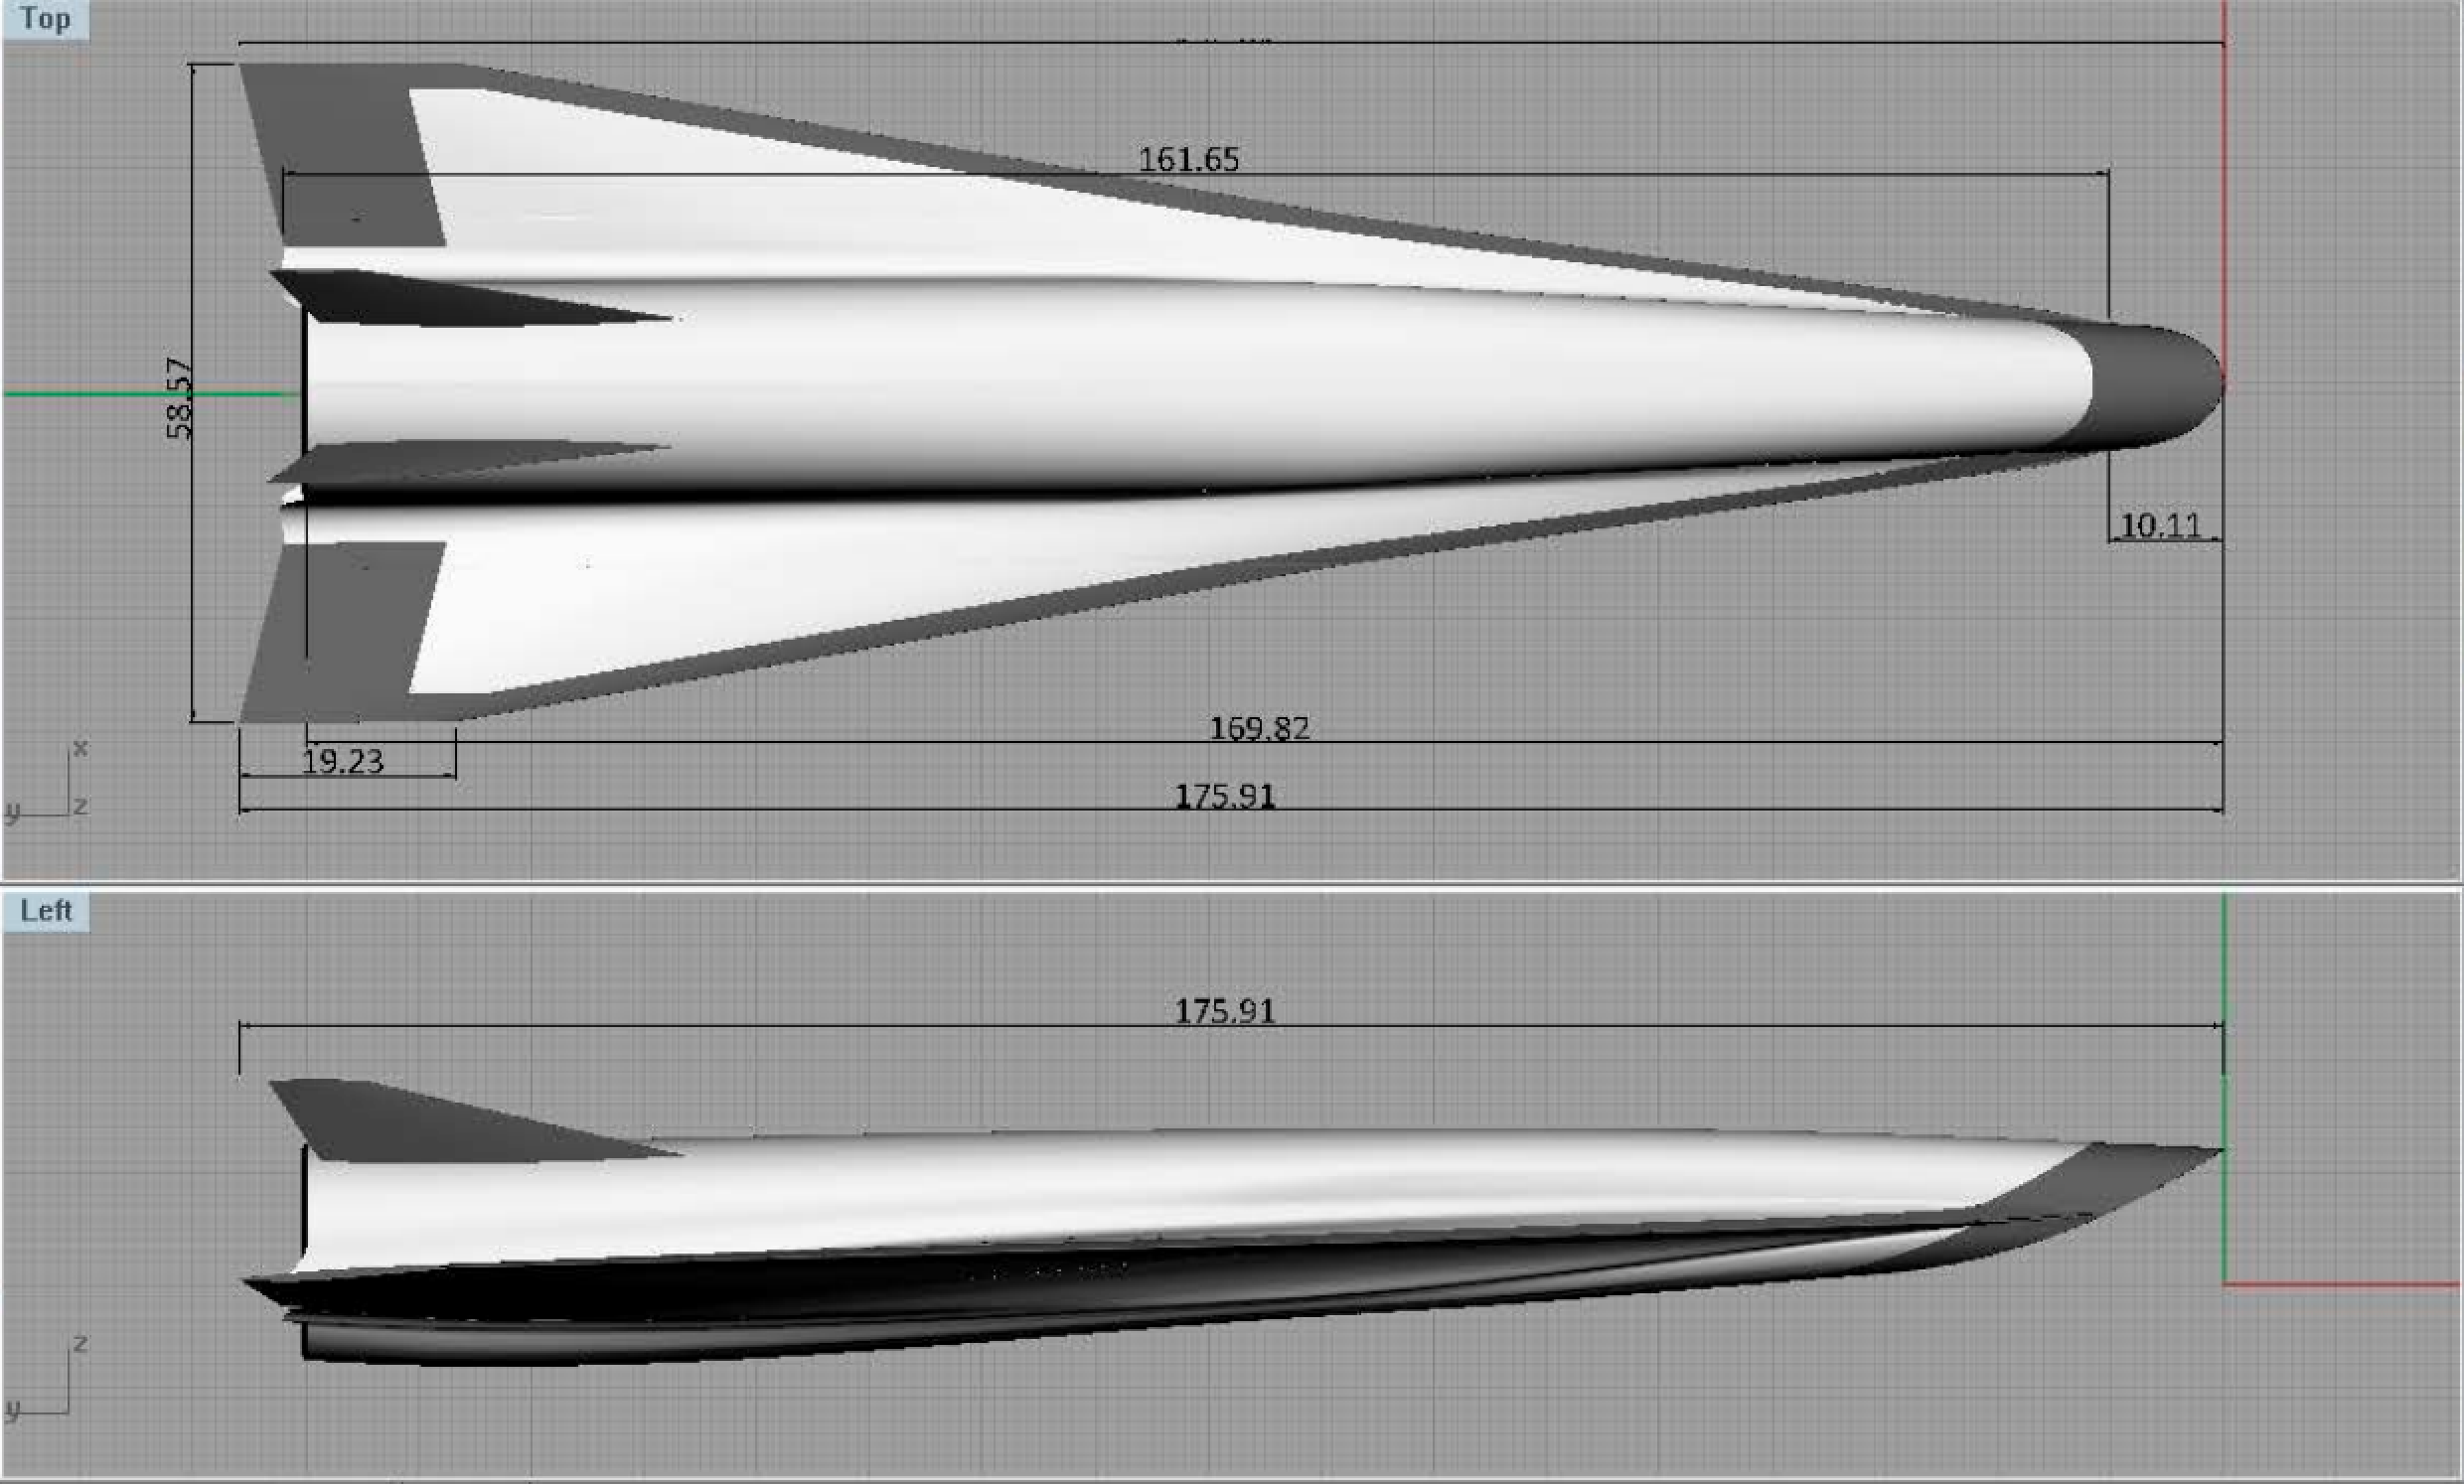
\includegraphics[width=4.5in]{\figurepath/ghvmodelview.png}
    \caption{AFRL Road Runner generic hypersonic vehicle\ \cite{ruttle.ghv.2012}\label{fig.ghvclouds}}
  \end{center}
\end{figure}

The Road Runner GHV was developed by AFRL in an effort to create a publicly releasable hypersonic vehicle model for studies of operability, controllability, and aero-propulsion integration as described in Reference\ \cite{ruttle.ghv.2012}.
The objective was to design a common vehicle which would be relevant to the technical efforts of current hypersonic projects, including the HIFiRE 6 vehicle, which the Road Runner closely resembles, as can be seen in Reference\ \cite{bolender.hifire6.2012}.
This GHV was designed be launched on rocket to accelerate it to cruise at Mach 6, at a dynamic pressure of between 1000--2000 psf.
The mission profile for the GHV then required maneuvers to be performed during the middle of the cruise phase before descending and decelerating, and making an unpowered maneuver to evaluate the potential to make a controlled landing.
The GHV should have the capability to perform sustained maneuvers up to a load factor of up to approximately 2G.

\begin{table}[H]
  \centering
  \caption{Vehicle properties}
  \begin{tabular}{llr}
    \toprule
    Parameter & Unit & Value \\
    \midrule
    Gross weight & [lbm] & $1220.3$ \\
    Empty weight & [lbm] & $993.3$ \\
    Vehicle length & [in] & $175.9$ \\
    Span & [in] & $58.6$ \\
    Nose diameter & [in] & $11.0$ \\
    Tail diameter & [in] & $18.8$ \\
    \bottomrule
  \end{tabular}\label{tab:vehicle_properties}
\end{table}

The aerodynamic data for the Road Runner was calculated using Hypersonic Engineering Aerothermodynamic Trajectory Tool Kit (HEAT-TK), developed for the Air Force by Boeing\ \cite{carter.heattk.2005}, and the engine data is calculated using the Ramjet Performance Analysis (RJPA) code, developed at Johns Hopkins University's Applied Physics Lab.

\section{Modeling the GHV}

The equations of motion describing many aircraft can be derived assuming a flat, non-rotating Earth.
Due to the high flight speed of a hypersonic vehicle in the atmosphere, the rotation and curvature of the Earth are typically significant, and should not be neglected.
Thus, the governing equations of motion for the GHV are derived assuming the vehicle is a rigid body flying through the atmosphere of a spherical, rotating Earth.
The equations of motion describing the GHV are given in References\ \cite{etkin.atmosphericflight.1972,billamoria.eom.1995}, and will be presented here for completeness.

\subsubsection*{Notation}

In deriving and applying the equations of motion which govern the motion of an aircraft, care must be taken to carefully book-keep the various vector quantities which describe the position, velocity and orientation of the aircraft.
For instance, when considering the velocity of an aircraft, it must be kept clear both with which frame the velocity is with respect to, and in which frame the velocity vector is described.
Some of the standard notation describing the expression of vectors in various reference frames is outlined below.
\begin{itemize}
  \item{$f_{a}$ denotes reference frame $a$.}
  \item{$O_{a}$ denotes the origin of reference frame $a$.}
  \item{$V^{a}_{b}$ describes the velocity of the origin of reference frame $b$ relative to the axes of reference frame $a$, described using the coordinate system of reference frame $b$.}
  \item{$\omega^{a,b}_{c}$ describes the angular velocity of reference frame $a$ relative to reference frame $b$ described using the axes of reference frame $c$. Omission of the second superscript implies the angular velocity of coordinate system $a$ is with respect to inertial axes. When the subscript is omitted, it is implied this quantity is described in the coordinates of frame $a$. For example $\omega^{B}$ is the inertial angular velocity of frame $f_{B}$, described using the axes of frame $f_{B}$.}
  \item{The transformation $R_{ab}$ describes a vector transformation from being expressed in reference frame $b$ to being expressed in reference frame $a$.}
  \item{$\frac{dV_{a}}{dt}\bigr|_{b}$ denotes the rate of change of $V_{a}$ with respect to frame $b$.}
  \item{All vectors are describing a relation of frame $a$ to frame $b$ are described along the axes of frame $a$.}
\end{itemize}

In many cases, the equations of motion can be greatly simplified when studying the dynamics of an aircraft.
Such simplifications often center around assuming the Earth is flat, but this may be an oversimplification for problems of hypersonic atmospheric flight.
While this simplification still might be acceptable for calculations involving the attitude dynamics where the rotating earth terms are typically very small, in trajectory calculations the rotating earth terms for a hypersonic vehicle become non-negligible.
This section presents the equations of motion that describe the GHV.\@

\subsection{Equations of Motion}

The equations of motion are developed using an Earth-centered, Earth-frame $f_{EC}$ with origin at the center of a spherical, rotating Earth.
It is assumed that the atmosphere travels uniformly with Earth as it rotates with angular velocity $\omega_{\text{earth}}$ in inertial space, and that the aircraft is sufficiently rigid that flexible structural effects can be neglected.
The position of the GHV around Earth and relative to $f_{EC}$ is described by its latitude $\lambda$, longitude $\tau$, and distance from the center of the Earth, $\mathscr{R}$.
These three coordinates give the location of the vehicle-carried frame $f_{V}$, defined with $z$-axis always pointing toward the origin of $f_{EC}$.

\begin{figure}[h]
  \begin{center}
    \small
    \psfrag{N}[bc][bc]{$N$}
    \psfrag{wE}[bl][bl]{$\omega_{\text{earth}}$}
    \psfrag{xE}[bc][bc]{$x_{E}$}
    \psfrag{yE}[bc][bc]{$y_{E}$}
    \psfrag{FE}[bc][bc]{$f_{E}$}
    \psfrag{OE}[bc][bc]{$O_{E}$}
    \psfrag{zEC}[bc][bc]{$z_{I}$}
    \psfrag{zE}[bc][bc]{$z_{E}$}
    \psfrag{yEC}[bc][bc]{$y_{I}$}
    \psfrag{FEC}[bc][bc]{$f_{I}$}
    \psfrag{OEC}[bc][bc]{$O_{I}$}
    \psfrag{xEC}[bc][bc]{$x_{I}$}
    \psfrag{lambda}[bl][bl]{$\lambda$}
    \psfrag{tau}[bc][bc]{$\tau$}
    \psfrag{eq}[bl][bl]{Equator}
    \psfrag{mer}[br][br]{Meridian}
    \psfrag{xv}[br][br]{$x_{V}$}
    \psfrag{yv}[bl][bl]{$y_{V}$}
    \psfrag{zv}[tr][tr]{$z_{V}$}
    \psfrag{ov}[tl][tl]{$O_{V}$}
    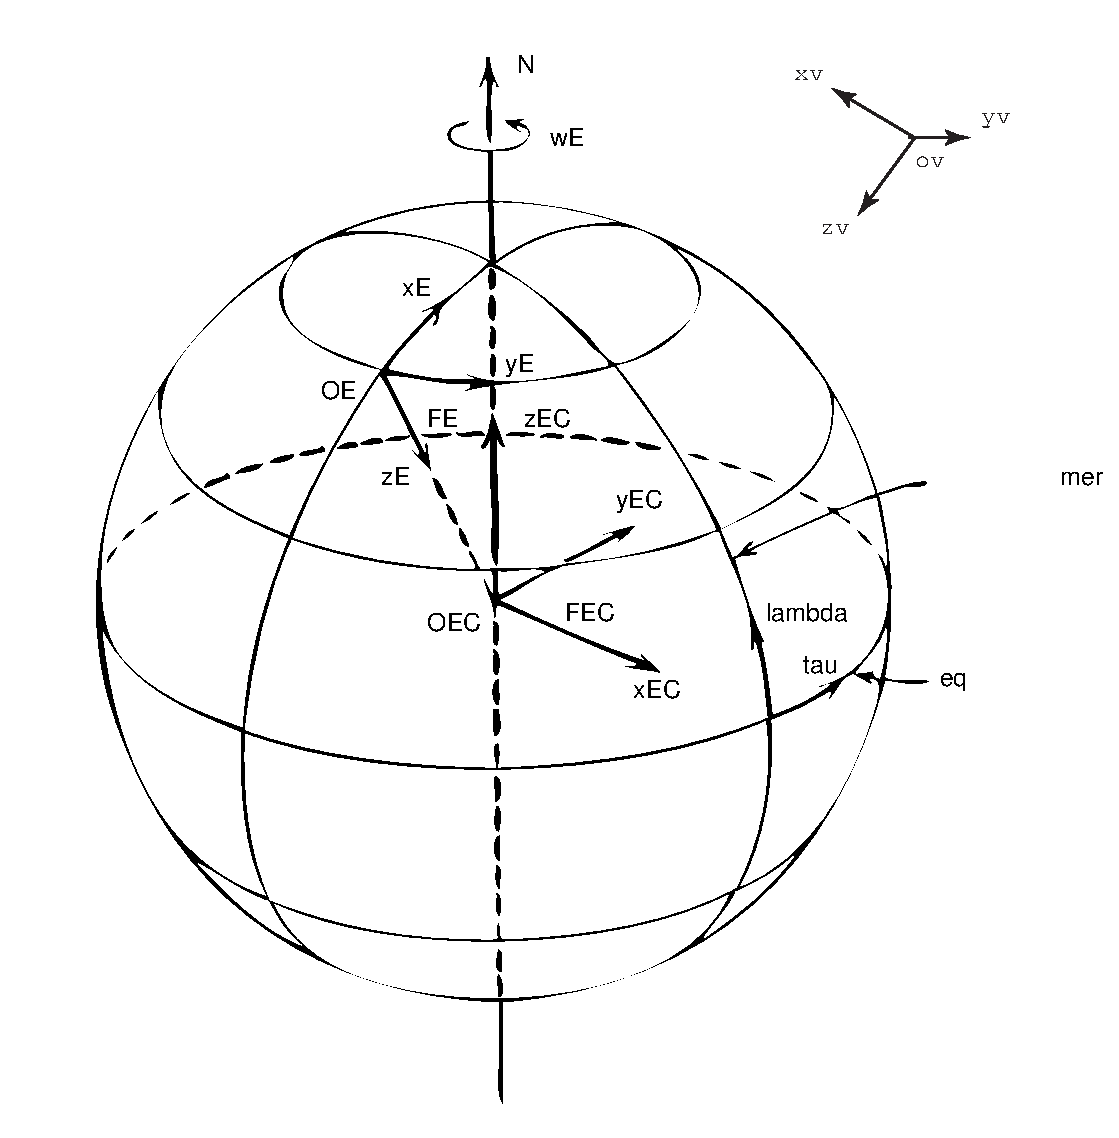
\includegraphics[height=3.5in]{\figurepath/earth_fig_4.eps}
    \caption{Reference frames\label{globe_fig}}
  \end{center}
\end{figure}

The vehicle carrying frame $f_{V}$ is a frame with origin attached to vehicle at the CG, and the z-axis $O_{V}z_{V}$ is defined to point vertically downward along the local $g$ vector.
$O_{V}x_{V}$ is defined to point north, and $O_{V}y_{V}$ east as shown in Figure~\ref{globe_fig}.
The vehicle-carried frame has angular velocity $\omega^{V}$ due to the curvature of the earth.
The body-fixed reference frame $f_{B}$ is a right-handed coordinate system attached to the GHV with $x$-axis pointing towards the nose of the aircraft along the longitudinal axis, and the $z$-axis pointing down.
This body-fixed axis system is used to derive the equations of motion for the GHV.\@

In deriving the equations of motion, the only additional assumption is that the centripetal acceleration due to $\omega_{\text{earth}}$ is negligible.
The equations of motion describe the dynamics of the GHV around the Earth when subject to external forces and moments.
These forces and moments, given in the body axes by $F_{B}$, and $M_{B}$ respectively, are due to the thrust and aerodynamic forces acting on the GHV, and are taken from pre-determined look-up tables within the simulation.
The aerodynamic forces depend on on control surface deflection angle, dynamic pressure, angle of attack, and sideslip angle.
The thrust forces depend on on control surface deflection angle, dynamic pressure, and angle of attack.

\subsubsection*{Force Equations}

The force equation describing the the motion of the GHV center of gravity in body axes is given as the following
\begin{equation}
  \label{eqn:forceeqn}
  \frac{dV^{A}_{B}}{dt}\biggr|_{B}+\omega^{B}\times V^{A}_{B}+
  \omega^{E}_{B}\times V^{A}_{B}+\omega^{E}_{B}\times(\omega^{E}_{B}\times\mathscr{R})=
  g+(F_{A}+F_{T})/m
\end{equation}
where $V^{A}_{B}$ denotes the velocity of $f_{B}$ relative to the atmosphere-fixed reference frame, and $\omega^{E}_{B}$ is the inertial angular velocity of the Earth-fixed frame $f_{E}$, described using the coordinate system of the body reference frame.
Note in this work that the atmosphere is assumed fixed with respect to the earth, so $f_{A}=f_{E}$.
The components of the atmospheric velocity are
\begin{equation}
  V_{B}^{A}=
  \bigr[
  \begin{array}{ccc}
    u & v & w
  \end{array}\bigr]^{\top}
\end{equation}
The force vector $F_{B}$ that represents all non-gravitational forces acting on the body in body axes is given by
\begin{equation}
  F_{B}=
  \bigr[
  \begin{array}{ccc}
    X & Y & Z
  \end{array}\bigr]^{\top}
\end{equation}
In the Equation (\ref{eqn:forceeqn}) this force is separated into aerodynamic and propulsive contributions as $F_{B}=F_{A}+F_{T}$ where the aerodynamic and propulsive forces have components given by
\begin{equation}
  \begin{split}
    F_{A}&=
    \bigr[
    \begin{array}{ccc}
      X_{A} & Y_{A} & Z_{A}
    \end{array}\bigr]^{\top} \\
    F_{T}&=
    \bigr[
    \begin{array}{ccc}
      X_{T} & Y_{T} & Z_{T}
    \end{array}\bigr]^{\top}
  \end{split}
\end{equation}

\subsubsection*{Moment equations}

The vehicle moments are described by the following equation.
Note the absence of any rotor contributions to the vehicle moment, as the scramjet engine lacks moving parts, unlike jet-turbine powered craft.
\begin{equation}
  \label{eqn:momenteqn}
  J\frac{d\omega^{B}}{dt}\biggr|_{B}+\omega^{B}\times J\omega^{B}=M_{A}+M_{T}
\end{equation}
$\omega_{B}$ is the angular velocity of the body frame relative to the inertial frame, with the rate of change evaluated in the body frame, and components
\begin{equation}
  \omega^{B}=
  \bigr[
  \begin{array}{ccc}
    p & q & r
  \end{array}\bigr]^{\top}
\end{equation}
The total torque in body axes is given by
\begin{equation}
  M_{B}=
  \bigr[
  \begin{array}{ccc}
    L & M & N
  \end{array}\bigr]^{\top}
\end{equation}
This total moment is split into the contributions due to aerodynamic and propulsive moments in Equation (\ref{eqn:momenteqn}) as $M_{B}=M_{A}+M_{T}$ where the aerodynamic and propulsive moments have components given by
\begin{equation}
  \begin{split}
    M_{A}&=
    \bigr[
    \begin{array}{ccc}
      L_{A} & M_{A} & N_{A}
    \end{array}\bigr]^{\top} \\
    M_{T}&=
    \bigr[
    \begin{array}{ccc}
      L_{T} & M_{T} & N_{T}
    \end{array}\bigr]^{\top}
  \end{split}
\end{equation}
The moment of inertia matrix $J$ is given by
\begin{equation}
  J=
  \begin{bmatrix}
    J_{xx} & -J_{xy} & -J_{xz} \\
    -J_{xy} & J_{yy} & -J_{yz} \\
    -J_{xz} & -J_{yz} & J_{zz}
  \end{bmatrix}
\end{equation}
Without any simplification, expansion of the moment equations would become very cumbersome.
In general, aircraft are symmetric about the $x-z$ plane, mass is uniformly distributed, and the body coordinate system is oriented such that $J_{xy}=J_{yz}=0$.
This allows the moment of inertia matrix for the GHV to be simplified to
\begin{equation}
  J=
  \begin{bmatrix}
    J_{xx} & 0 & -J_{xz} \\
    0 & J_{yy} & 0 \\
    -J_{xz} & 0 & J_{zz}
  \end{bmatrix}
\end{equation}

\subsubsection*{Orientation Equations}

The orientation, or kinematic equations describe the orientation of the aircraft body axes with respect to the vehicle carried frame.
The relationship between Euler rates and body angular velocities in the vehicle- carried frame is given by

\begin{equation}
  \label{eulr_ss_eqn}
  \left[
  \begin{array}{c}
    \dot{\phi} \\
    \dot{\theta} \\
    \dot{\psi}
  \end{array}\right]=
  \left[
  \begin{array}{ccc}
    1 & \tan(\theta)\sin(\phi) & \tan(\theta)\cos(\phi) \\
    0 & \cos(\phi) & -\sin(\phi) \\
    0 & \sin(\phi)/\cos(\theta) & \cos(\phi)/\cos(\theta)
  \end{array}\right]
  \left[
  \begin{array}{c}
    p_{v} \\
    q_{v} \\
    r_{v}
  \end{array}\right]
\end{equation}
where $\phi$, $\theta$, and $\psi$ are the roll, pitch, and yaw or heading angles, respectively, and are known as the Euer angles.
The components of angular velocities $p_{v}$, $q_{v}$, and $r_{v}$ are for the aircraft with body-fixed reference frame $f_{B}$ and are relative to the vehicle-carrying frame $f_{V}$.
These components of angular velocity are about the $x$, $y$, and $z$ body axes, respectively.
The relative angular velocities of the GHV are related to the vehicle absolute angular velocities by
\begin{equation}
  \begin{bmatrix}
    p_{v} \\
    q_{v} \\
    r_{v}
  \end{bmatrix}=
  \begin{bmatrix}
    p \\
    q \\
    r
  \end{bmatrix}-R_{BV}
  \begin{bmatrix}
    (\omega_{\text{earth}}+\dot{\tau})\cos{\lambda} \\
    -\dot{\lambda} \\
    -(\omega_{\text{earth}}+\dot{\tau})\sin{\lambda}
  \end{bmatrix}
\end{equation}
where $R_{BV}$ is the orthogonal rotation matrix given by
\begin{equation}
  R_{BV}=
  \begin{bmatrix}
    \cos{\theta}\cos{\psi} & \cos{\theta}\sin{\psi} & -\sin{\theta} \\
    \sin{\phi}\sin{\theta}\cos{\psi}-\cos{\phi}\sin{\psi} & \sin{\phi}\sin{\theta}\sin{\psi}+\cos{\phi}\cos{\psi} & \sin{\phi}\cos{\theta}\\
    \cos{\phi}\sin{\theta}\cos{\psi}+\sin{\phi}\sin{\psi} & \cos{\phi}\sin{\theta}\sin{\psi}-\sin{\phi}\cos{\psi} & \cos{\phi}\cos{\theta}
  \end{bmatrix}
\end{equation}

The reason for the distinction between relative and absolute angular rates in the above equations is due to the spherical Earth.
If a hypersonic vehicle was flying continuous circles around the world, the Euler rate's would all be zero as the aircraft would be stationary relative to the vehicle carried frame.
However, the absolute angular rates would be non-zero, as the vehicle carried frame would be rotating as it moved over the surface of the Earth.

\subsubsection*{Navigation Equations}

The location, or navigation equations describe the location of the origin of the body fixed coordinate system with respect to the inertial axes.
The quantities describing this location are latitude, longitude, and altitude.
The navigation kinematic equation is given by
\begin{equation}
  \begin{bmatrix}
    \dot{\lambda}\mathscr{R} \\
    \dot{\tau}\mathscr{R}\cos{\lambda} \\
    -\dot{\mathscr{R}}
  \end{bmatrix}=R_{VB}
  \begin{bmatrix}
    u \\
    v \\
    w
  \end{bmatrix}
\end{equation}
where $R_{VB}=R_{BV}^{-1}$.

\subsubsection*{Construction of Equations}

These equations were assembled in a \textsc{Simulink} model with main component blocks as indicated in Figure~\ref{fig.ghvblocks}.
The forces and moments are calculated from aerodynamic and engine data stored in look-up tables.

\begin{figure}[H]
  \begin{center}
    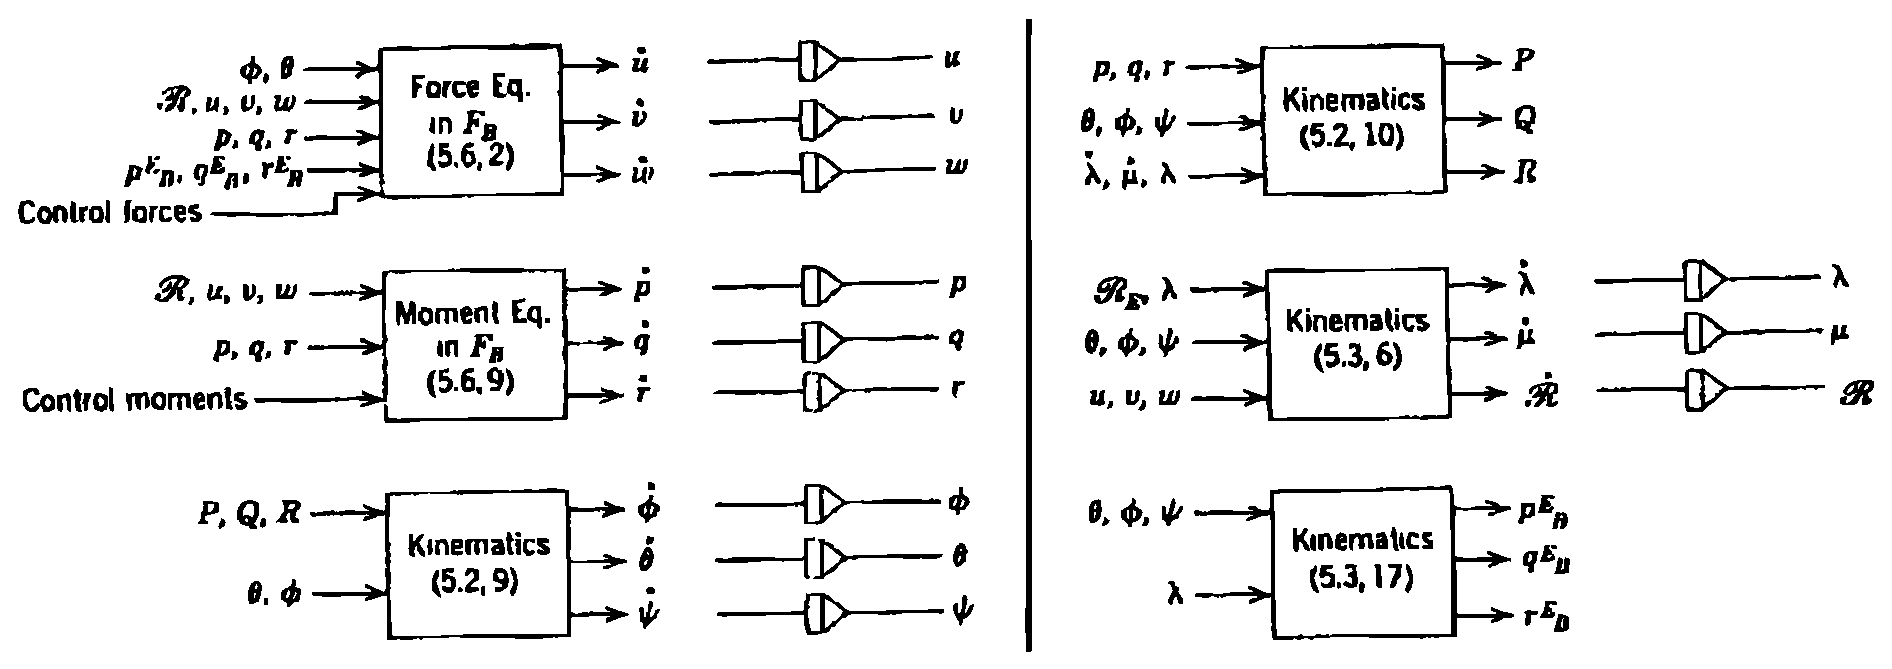
\includegraphics[width=6.0in]{\figurepath/block_eqns_2.eps}
    \caption{Equation of motion model blocks\ \cite{etkin.atmosphericflight.1972}\label{fig.ghvblocks}}
  \end{center}
\end{figure}

\section{State Space Representation}

The equations of motion can be represented in state-space form as
\begin{equation}
  \dot{X}=f({X},U)
\end{equation}
with state vector
\begin{equation}
  \label{eqn:fullstatevectorx}
  X=\left[
  \begin{array}{cccccccccccc}
    V_{T} &  \alpha & q &\theta & h & \beta &p & r & \phi &\psi &\lambda & \tau
  \end{array}\right]^{\top}
\end{equation}
where $V_{T}$ is the total velocity, $\alpha$ and $\beta$ are the angle of attack and sideslip angle, $\phi$, $\theta$, and $\psi$ are the roll, pitch, and yaw angles, $p$, $q$, and $r$ are the absolute angular velocity components, and $\lambda$, $\tau$, and $h$ are the latitude, longitude, and altitude, of the GHV, respectively.
The input vector is given by
\begin{equation}
  \label{eqn:fullcontrolvector}
  U=\left[
  \begin{array}{cccc}
    u_{\text{th}} & u_{\text{elv}} & u_{\text{ail}} & u_{\text{rud}}
  \end{array}\right]^{\top}
\end{equation}
where $u_{\text{th}}$, $u_{\text{elv}}$, $u_{\text{ail}}$, and $u_{\text{rud}}$ are the throttle, elevator, aileron, and throttle inputs, respectively.
The entries of the state vector are arranged so as to facilitate separation of the lateral and longitudinal equations of motion during control design.
The deflection of the elevons are accomplished through static mixing, combining differential and collective deflections from the aileron and elevator commands, respectively, while both rudders are actuated together using the single rudder input.
The control vector $U_{5}$ contains the deflections of the right and left elevons ($u_{r,\text{elv}}$, $u_{l,\text{elv}}$), rudders ($u_{r,\text{rud}}$, $u_{l,\text{rud}}$), and throttle as
\begin{equation}
  U_{5}=
  \bigr[
  \begin{array}{ccccc}
    u_{\text{th}} & u_{r,\text{elv}} & u_{l,\text{elv}} & u_{r,\text{rud}}  & u_{l,\text{rud}}
  \end{array}\bigr]^{\top}
\end{equation}
The control allocation matrix $M$ is the matrix which defines the following transformation between control vectors $U_{5}$ and $U$ as
\begin{equation}
  U=MU_{5}
\end{equation}
where control allocation matrix is
\begin{equation}
  M=
  \left[
  \begin{array}{ccccc}
    1 & 0 & 0 & 0 & 0 \\
    0 & 1/2 & 1/2 & 0 & 0 \\
    0 & 1/2 & -1/2 & 0 & 0 \\
    0 & 0 & 0 & 1/2 & 1/2 \\
  \end{array}\right]
\end{equation}

\subsection{Actuator and Sensor Models}

\paragraph{Throttle} The propulsion system is modeled as a first order system with a cutoff frequency of 10 rad/s, with transfer function
\begin{equation*}
  G_{\text{th}}(s)=\frac{\omega_{\text{th}}}{s+{\omega_{\text{th}}}}
\end{equation*}
While the physics of the engine happen on time scales order of magnitude faster than the rest of the dynamics, this simple model was proposed to capture fuel system delivery limits.

\paragraph{Control Surfaces} Second order actuators with rate and deflection limits were included in the simulation model on all four of the aerodynamic control surfaces.
The transfer function for the control surface actuators is
\begin{equation}
  G_{\text{cs}}(s)=\frac{{\omega_{n}}^{2}}{s^{2}+2\zeta\omega_{n}s+{\omega_{n}}^{2}}
\end{equation}
and the block diagram for the control surfaces as implemented is shown in Figure~\ref{fig:actuator_block} where the signal $u_{\text{cmd}}$ is generated by the controller, and due to the actuator dynamics the actual control surface deflection is given by $u_{\text{sat}}$.

\begin{figure}[H]
  \begin{center}
    \begin{tikzpicture}[auto, scale=0.9, every node/.style={transform shape}, node distance=1.5cm, >=latex']
    \node[input](input1){};
    \node[satnode,draw,fill=white, minimum height=1.0cm, minimum width=1.0cm, right of=input1, node distance=1.5cm, label=below:{\shortstack{deflection \\ saturation}}] (block1){};
    \node[whitesum, right of=block1,node distance=1.8cm](sum1){$+$};
    \node[squareblock, right of=sum1,node distance=1.8cm] (block2){$\omega_{n}^{2}$};
    \node[whitesum, right of=block2, node distance=1.8cm](sum2){$+$};
    \node[squareblock, right of=sum2,node distance=1.8cm] (block3){$\frac{1}{s}$};
    \node[satnode,draw,fill=white, minimum height=1.0cm, minimum width=1.0cm, right of=block3, node distance=2.5cm, label=below:{\shortstack{rate \\ saturation}}] (block4){};
    \node[squareblock, right of=block4,node distance=2.0cm] (block5){$\frac{1}{s}$};
    \node[satnode,draw,fill=white, minimum height=1.0cm, minimum width=1.0cm, right of=block5, node distance=2.0cm, label=below:{\shortstack{deflection \\ saturation}}] (block6){};
    \node[output, right of=block6,node distance=1.5cm] (output1) {};
    \node[squareblock, below of=block3,node distance=2.0cm] (block7){$2\zeta\omega_{n}$};
    \node[tee,below of=block7,node distance=1.5cm] (tee1){};
    %Draw lines
    \draw[->](input1) -- node[near start]{$u_{\text{cmd}}$} (block1);
    \draw[->](block1) -- node[near end]{$+$} (sum1);
    \draw[->](sum1) -- (block2);
    \draw[->](block2) -- node[near end]{$+$} (sum2);
    \draw[->](sum2) -- node{$\ddot{u}$} (block3);
    \draw[->](block3) -- node[pos=0.4,name=u]{$\dot{u}$} (block4);
    \draw[->](block4) -- (block5);
    \draw[->](block5) -- node[pos=0.4,name=y]{$u$} (block6);
    \draw[->](block6) -- node[near end]{$u_{\text{sat}}$} (output1);
    \draw[->](u) |- (block7);
    \draw[->](block7) -| node[pos=0.95]{$-$} (sum2);
    \draw[-](y) |- (tee1);
    \draw[->](tee1) -| node[pos=0.95]{$-$} (sum1);
    \end{tikzpicture}
    \caption{Second order actuator block diagram\label{fig:actuator_block}}
  \end{center}
\end{figure}

The relevant values used in the second order aerodynamic control surface actuator model are listed in Table~\ref{tab:actuator}.
\begin{table}[H]
  \centering
  \caption{Second order aerodynamic control surface actuator parameters\label{tab:actuator}}
  \begin{tabular}{llc}
    \toprule
    Parameter & Unit & Value \\
    \midrule
    Elevon deflection limit & [deg] & $-30$ to $30$ \\
    Rudder deflection limit & [deg] & $-30$ to $30$ \\
    Elevon rate limit & [deg/s] & $-100$ to $100$ \\
    Tail rate limit & [deg/s] & $-100 $ to $100$ \\
    Damping ratio $\zeta$ & & $0.7$ \\
    Natural frequency $\omega_{n}$ & [rad/s] & $150$ \\
    \bottomrule
  \end{tabular}
\end{table}

\paragraph{Sensor Filters} First order low-pass filters were placed at the sensor outputs in order to model the effects of a navigation filter in the loop, and reduce sensor noise being fed back to the controller.
The velocity filter has a cutoff frequency of 20 rad/s, while the incidence, angular rate, and Euler angle sensor filters all have a cutoff frequency of 150 rad/s.

\subsection{Implementation}

The GHV simulation block diagram is in Figure~\ref{fig:ghvcontrolblock}.
The controller was implemented in discrete time and operated at 100 Hz with a zero-order hold on the control signal output.
The output sensors are operated at 600 Hz also using zero-order hold samping, white noise was injected into the sensor signals, and a variable input time delay was used.

\begin{figure}[H]
  \begin{center}
    \begin{tikzpicture}[auto, scale=0.8, every node/.style={transform shape}, node distance=1.0cm, >=latex']
    \node[squareblock, minimum height=1cm, minimum width=2cm, label=below:{100 Hz}] (block1){Controller};
    \node[input,left=of block1.170, node distance=2.0cm] (j1) {};
    \node[left of=j1, node distance=0.5cm] (input1) {};
    \node[input,left=of block1.190, node distance=1.0cm] (input2) {};
    \node[squareblock, minimum width=1cm, right of=block1, node distance=2.5cm] (block2) {$\tau_{\text{delay}}$};
    \node[squareblock, minimum height=1cm, minimum width=1.0cm, label=below:{\shortstack[c]{Actuator\\Dynamics}}, right of=block2,node distance=2.5cm, inner sep= 1mm] (block3) {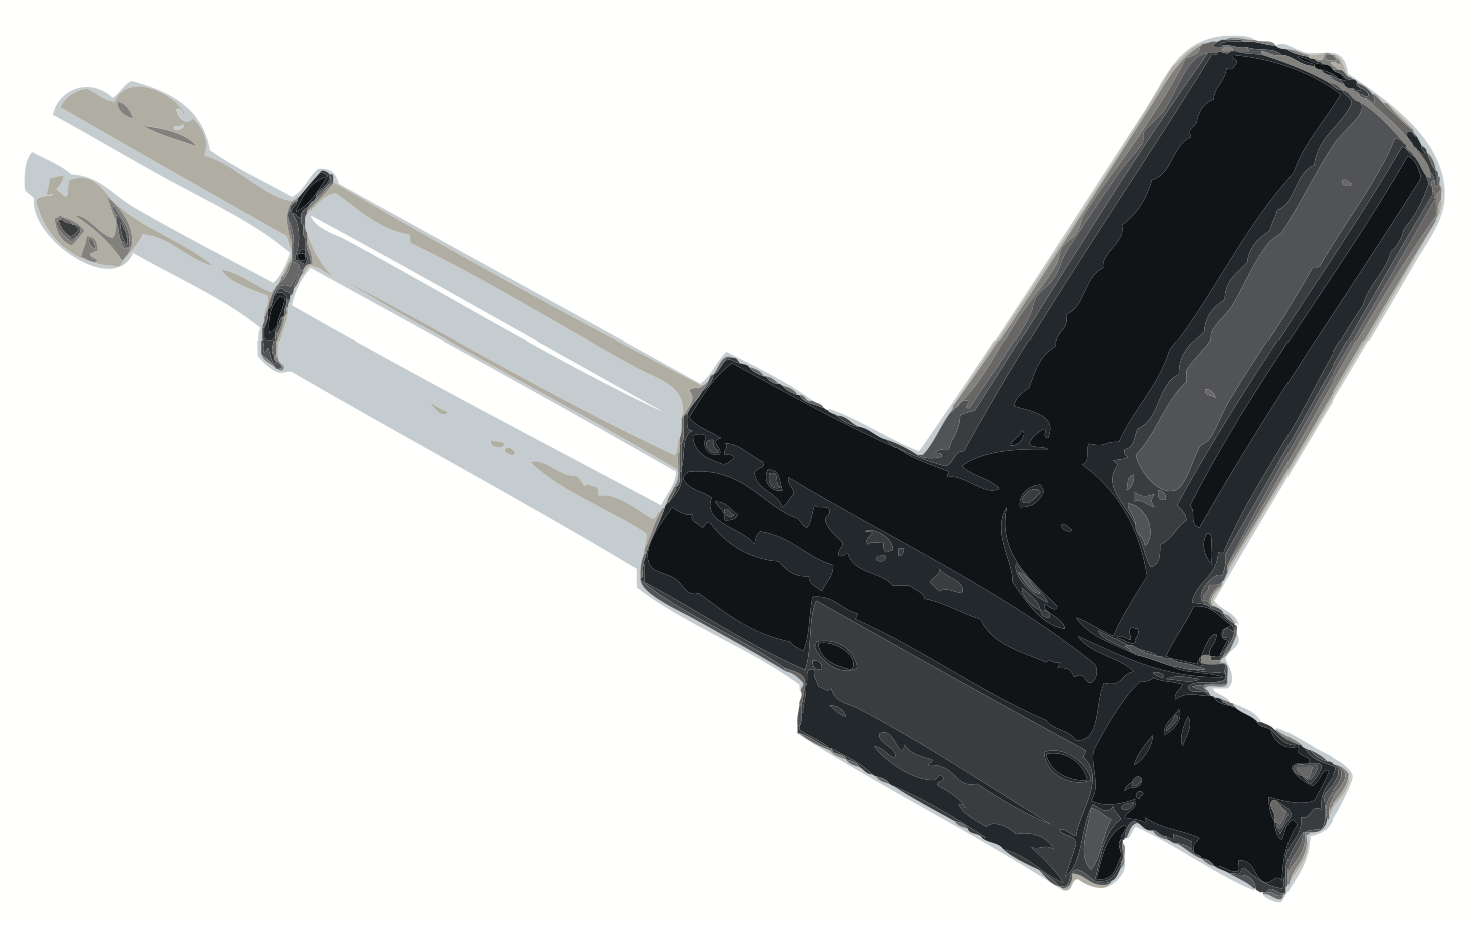
\includegraphics[width=1.6cm]{\figurepath/actuator_image.png}};
    \node [right of=block3,draw=black, anchor=west,node distance=2.0cm, minimum width=2cm, label=below:{Plant}, inner sep= 0mm] (block4) {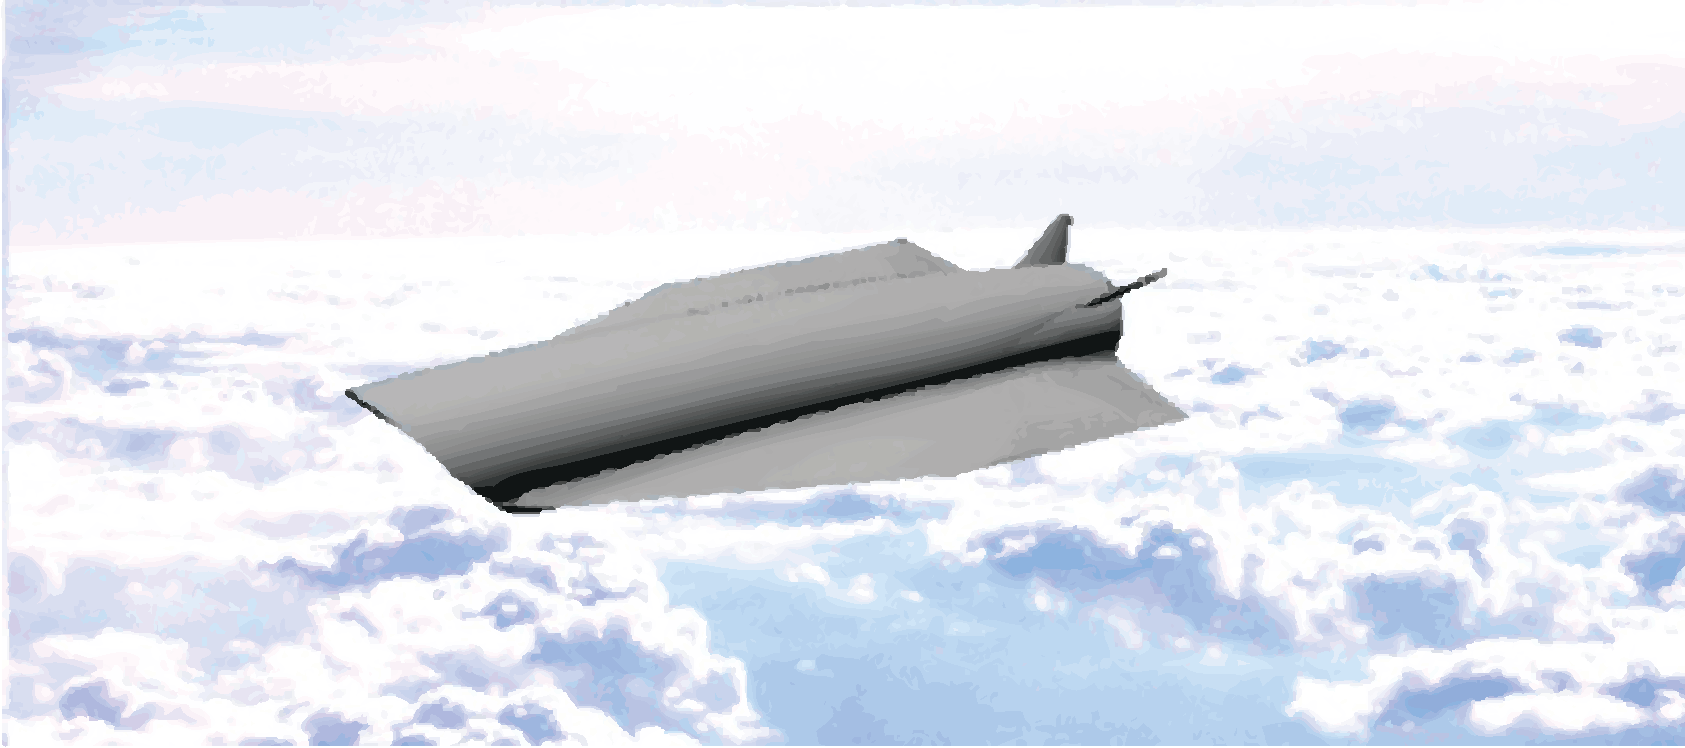
\includegraphics[width=4cm]{\figurepath/ghvclouds.pdf}};
    \node[whitesum, right of=block4,node distance=3.0cm] (sum1) {$+$};
    \node[input, above of=sum1,node distance=1.2cm](input3){};
    \node[squareblock, minimum width=1cm, right of=sum1, node distance=2.0cm] (block5) {ZOH};
    \node[squareblock, minimum width=1cm, right of=block5, node distance=2.0cm] (block6) {Filter};
    \node[output, right of=block6,node distance=2.0cm] (output1) {};
    \node[tee, below of=block3,node distance=1.8cm](tee1){};
    %Draw lines
    \draw[-](input1) -- node[near start]{$z_{\text{cmd}}$} (j1);
    \draw[->](j1) -- (block1.170);
    \draw[->](input2) -- (block1.190);
    \draw[->](block1) -- (block2);
    \draw[->](block2) -- (block3);
    \draw[->](block3) -- (block4);
    \draw[->](block4) -- (sum1);
    \draw[->](input3) -- (sum1);
    \draw[->](sum1) -- (block5);
    \draw[->](block5) -- node[name=n,pos=0.5]{}(block6);
    \draw[->](block6) -- node[name=y,pos=0.7]{} node[near end]{$x$}(output1);
    \draw[-](y) |- node[pos=0.9] {} (tee1);
    \draw[-](tee1) -| (input2);
    %Model box
    \begin{pgfonlayer}{background}
      \path (block5 |- block5)+(-1.0,0.7) node (c) {};
      \path (block6 -| block6)+(1.0,-0.7) node (d) {};
      \path[fill=gray!20, draw, dashed] (c) rectangle (d);
    \end{pgfonlayer}
    \node [above of=sum1, node distance = 1.5cm] {noise};
    \node[below of=n,node distance=1.2cm]{600 Hz};
    \end{tikzpicture}
    \caption{GHV flight control simulation block diagram\label{fig:ghvcontrolblock}}
  \end{center}
\end{figure}

The discretization of the controller and sensor models as well as the addition of time delay, actuator dynamics, and noise makes the evaluation model a more realistic representation of the actual hardware on which the proposed control laws would be implemented.
This is to better evaluate through simulations the robustness capability of the control design as it contends with these realistic effects.

\section{Open-Loop Analysis}

The open-loop behavior of the GHV was analyzed about a nominal flight condition of $M=6$, $h=80,000$ ft, corresponding to a dynamic pressure of 1474 psf.
The geographical coordinates and heading of the GHV are insignificant in the equations of motion for the purposes of inner-loop control law development, and these state variables are dropped from the state vector (\ref{eqn:fullstatevectorx}) for trim, linearization, and control.
\begin{equation}
  \label{eqn:truncstatevectorx}
  X=\bigr[
  \begin{array}{ccccccccc}
    V_{T} &  \alpha & q &\theta & h & \beta &p & r & \phi
  \end{array}\bigr]^{\top}
\end{equation}
The state $X$ from this point forward is used to mean the truncated state (\ref{eqn:truncstatevectorx}), as it contains the primary quantities describing the vehicle dynamics that are to be controlled.
The navigation components of (\ref{eqn:fullstatevectorx}) will evolve as a consequence of controlling (\ref{eqn:truncstatevectorx}) and in practice would be commanded through an outer-loop guidance controller.
The dynamics of the system with truncated state are described by
\begin{equation}
  \label{eqn:xdotfxu}
  \dot{X}=f({X},U)
\end{equation}
The equilibrium, or trim state $X_{\text{eq}}$ and input $U_{\text{eq}}$ satisfy
\begin{equation}
  \label{eqn:eqptdef}
  \dot{X}_{\text{eq}}=f({X}_{\text{eq}},U_{\text{eq}})=0
\end{equation}
The equilibrium state and input are found for the nominal steady, level cruise condition, and Equation (\ref{eqn:xdotfxu}) is linearized about this trim condition as follows.
Defining $x$ and $u$ to be state and input perturbations about equilibrium, the state and input can be expressed as
\begin{equation}
  \begin{split}
    X&=X_{\text{eq}}+x \\
    U&=U_{\text{eq}}+u
  \end{split}
\end{equation}
Differentiating (\ref{eqn:xdotfxu})
\begin{equation}
  \begin{split}
    \dot{X}=\dot{x}&=f(X, U) \\
    &=f(X_{\text{eq}}+x,U_{\text{eq}}+u)
  \end{split}
\end{equation}
Performing a Taylor series expansion, neglecting second order terms and higher
\begin{equation*}
  \dot{x}= f(X_{\text{eq}},U_{\text{eq}})+\left.\frac{\partial f(X,U)}{\partial X}\right|_{\text{eq}}x+\left.\frac{\partial f(X,U)}{\partial U}\right|_{\text{eq}}u+\epsilon
\end{equation*}
where the subscript $(\cdot)_{\text{eq}}$ indicates these quantities be evaluated at the equilibrium point.
With $f(X_{\text{eq}},U_{\text{eq}})=0$, the linearization results in the state-space system given by
\begin{equation}
  \label{eqn:linss}
  \dot{x}=Ax+Bu
\end{equation}
where
\begin{equation}
  A=\left.\frac{\partial f(X,U)}{\partial X}\right|_{\text{eq}}^{}
  \hspace{0.5in}
  B=\left.\frac{\partial f(X,U)}{\partial U}\right|_{\text{eq}}^{}
\end{equation}
Using this linear system, the open-loop dynamic modes of the GHV during the nominal steady level cruise condition are analyzed through a sensitivity analysis.
It is also important to note that the perturbation state $x$ of the linear system in Equation (\ref{eqn:linss}) will be represented as having the following components.
\begin{equation}
  x=\bigr[
  \begin{array}{ccccccccc}
    \Delta V_{T} & \Delta\alpha & \Delta q & \Delta\theta & \Delta h & \Delta\beta & \Delta p & \Delta r & \Delta\phi
  \end{array}\bigr]^{\top}
\end{equation}
The perturbation input for the linear system is equivalently defined as
\begin{equation}
  u=\left[
  \begin{array}{cccc}
    \Delta\delta_{\text{th}} & \Delta\delta_{\text{elv}} & \Delta\delta_{\text{ail}} & \Delta\delta_{\text{rud}}
  \end{array}\right]^{\top}
\end{equation}
In following sections, this notation is abused by not explicitly including the $\Delta$ preceding each component to indicate that the components of the state vector $x$ and input vector $u$ are in fact perturbation states and inputs, respectively.
This is done only when there is no possibility of confusion, and so when referring to the state and control input of the linear system given by Equation (\ref{eqn:linss}) the following notation will be used
\begin{equation}
  \label{eqn:perturbedstatevectorx}
  x=\bigr[
  \begin{array}{ccccccccc}
    V_{T} & \alpha & q &\theta & h & \beta &p & r & \phi
  \end{array}\bigr]^{\top}
\end{equation}
\begin{equation}
  u=\left[
  \begin{array}{cccc}
    \delta_{\text{th}} & \delta_{\text{elv}} & \delta_{\text{ail}} & \delta_{\text{rud}}
  \end{array}\right]^{\top}
\end{equation}

\subsection{Modal Analysis}

Given a linear system such as Equation (\ref{eqn:linss}) it is often of interest to examine the system modes.
Conventional aircraft usually have modes which are quite predictable in their characteristics from one vehicle to the next, but with an aircraft such as the GHV, the significant state variables in the different modes may differ from those of conventional aircraft.
Because of this it is crucial to analyze the system modes to better understand the dynamics of the GHV, and to facilitate the control design process.

The sensitivity matrix for the linear system given in Equation (\ref{eqn:linss}) is calculated, which contains the desired modal information.
The sensitivity analysis aims to determine which entries in a given eigenvector are small when the units of each state variable are not the same.
This method examines slight changes in the initial condition of each state separately in order to determine whether this change will influence some modes more strongly than others.
This analysis will provide knowledge of what modes the GHV exhibits, which states are dominant in each of these modes, as well as the stability of these modes.

\subsubsection*{Mode Sensitivity}
Consider the linear system (\ref{eqn:linss}) describing the GHV dynamics, with perturbation state vector given by (\ref{eqn:perturbedstatevectorx}).
This section outlines the method presented in\ \cite{etkin.atmosphericflight.1972} of applying a linear transformation to a state space system to obtain a system represented in characteristic coordinate system to facilitate the modal analysis and calculation of the sensitivity matrix.
Considering only the initial condition response, the following autonomous system results
\begin{equation}
  \label{eqn:xdotax}
  \dot{x}=Ax
\end{equation}
The following nonsingular transformation is introduced
\begin{equation}
  x=\mathbb{V}q
\end{equation}
where $\mathbb{V}\triangleq[\begin{array}{ccc} \mathrm{v}_{1} & \cdots & \mathrm{v}_{n} \end{array}]$ is the modal matrix made up of the eigenvectors or $A$ as shown.
Note that this transformation will not alter the eigenvalues or eigenvectors of the system in (\ref{eqn:xdotax}).
Using this transformation
\begin{equation}
  \dot{q}=\tilde{A}q
\end{equation}
where
\begin{equation}
  \tilde{A}=\mathbb{V}^{-1}A\mathbb{V}
\end{equation}
The matrix $\mathbb{V}^{-1}A\mathbb{V}$ can be expressed as
\begin{equation}
  A\mathbb{V}
  =A \left[
  \begin{array}{ccc}
    \mathrm{v}_{1} & \cdots & \mathrm{v}_{n}
  \end{array} \right]
  =\left[
  \begin{array}{ccc}
    A\mathrm{v}_{1} & \cdots & A\mathrm{v}_{n}
  \end{array}\right]
  =\left[
  \begin{array}{ccc}
    \mathrm{v}_{1}\lambda_{1} & \cdots & \mathrm{v}_{n}\lambda_{n}
  \end{array}\right]
  =\mathbb{V}\Lambda%
\end{equation}
giving
\begin{equation}
  \dot{q}=\Lambda{q}
\end{equation}
where $\Lambda$ is the diagonal matrix of eigenvalues.
The solution is given by
\begin{equation}
  q(t)=e^{\Lambda{t}}q(0)
\end{equation}
The unforced response of the system in response to initial conditions is of interest.
In particular, an initial condition is selected as a scalar multiple of an eigenvector $\mathrm{v}_{i}$
\begin{equation}
  x(0)=\alpha_{i}\mathrm{v}_{i}
\end{equation}
Using the linear transformation
\begin{equation}
  q(0)=\mathbb{V}^{-1}x(0)=\alpha_{i}\mathbb{V}^{-1}\mathrm{v}_{i}
\end{equation}
Since $\mathbb{V}^{-1}\mathbb{V}=\mathbb{I}$ where $\mathbb{I}$ is the identity matrix, $\mathbb{V}^{-1}\mathrm{v}_{i}$ is just the $\mathrm{i^{th}}$ column of $\mathbb{I}$.
In other words, the initial condition $q(0)$ corresponding to the selected $x(0)$ will be a column vector of zeros, with the exception of the entry $\alpha_{i}$ in the $\mathrm{i^{th}}$ row.
The response of the state $x(t)$ from this initial condition is given by
\begin{equation}
  \begin{split}
    x(t)&=\mathbb{V}e^{\Lambda{t}}\alpha_{i}\mathbb{V}^{-1}\mathrm{v}_{i} \\
    &=\alpha_{i}\mathbb{V}e^{\Lambda{t}}
    \bigr[
    \begin{array}{ccccc}
      0 & \hdots & 1 & \hdots & 0
    \end{array}\bigr]^{\top}
  \end{split}
\end{equation}
Expanding
\begin{equation}
  \begin{split}
    x(t)&=\alpha_{i}
    \left[
    \begin{array}{ccc}
      \mathrm{v}_{1} & \cdots & \mathrm{v}_{n}
    \end{array} \right]
    \left[
    \begin{array}{cccc}
      e^{\lambda_{1}t} & 0 & \cdots & 0 \\
      0 & e^{\lambda_{2}t} & \cdots & 0 \\
      \vdots & \vdots & \ddots & \vdots \\
      0 & 0 & \cdots & e^{\lambda_{n}t}
    \end{array}\right]
    \begin{bmatrix}
      0 \\
      \vdots \\
      1 \\
      \vdots \\
      0
    \end{bmatrix} \\
    &=\alpha_{i}e^{\lambda_{i}t}\mathrm{v}_{i}
  \end{split}
\end{equation}
This shows that only the mode corresponding to $\lambda_{i}$ will be present in the response from an initial condition along the $\mathrm{i^{th}}$ eigenvector.
The general response in terms of $x$ is given by summing the individual responses starting from each eigenvector initial condition
\begin{equation*}
  x(t)=\sum \limits_{i=1}^{n} \alpha_{i}e^{\lambda_{i}t}\mathrm{v}_{i}
\end{equation*}
Based on this unforced modal response, if any entries in $\mathrm{v}_{i}$ are small relative to the others, the corresponding states are thus not influential in determining the initial condition response.

\subsubsection*{Calculating the Sensitivity Matrix}

In this section the methods of\ \cite{manual.durham.2002} used to calculate the sensitivity matrix for $\tilde{A}$ are outlined.
The matrix $\mathbb{V}$ and its inverse $\mathbb{V}^{-1}$ are first calculated.
The rows of $\mathbb{V}$ are denoted using $r_{i}$, and the columns of $\mathbb{V}^{-1}$ as $c_{i}$
\begin{equation*}
  \mathbb{V}=
  \bigr[
  \begin{array}{cccc}
    r_{1}^{\top} & r_{2}^{\top} & \hdots & r_{n} ^{\top}
  \end{array}\bigr]^{\top}
  \hspace{0.5in}
  \mathbb{V}^{-1}=\left[
  \begin{array}{cccc}
    c_{1} & c_{2} & \cdots & c_{n}
  \end{array}\right]
\end{equation*}
The diagonal matrices $C_{i}$ are formed using the elements of $c_{i}$
\begin{equation*}
  c_{i}=\left[
  \begin{array}{c}
    c_{i,1} \\
    c_{i,2} \\
    \vdots \\
    c_{i,n}
  \end{array}\right] \hspace{0.5in}
  C_{i}=\left[
  \begin{array}{cccc}
  c_{i,1} & 0 & \cdots & 0 \\
  0 & c_{i,2} & \cdots & 0 \\
  \vdots & \vdots & \ddots & \vdots \\
  0 & 0 & \cdots & c_{i,n}
  \end{array}\right]
\end{equation*}
The $n \times n$ sensitivity matrix $S$ is defined as
\begin{equation*}
  S\equiv\left[
  \begin{array}{c}
    r_{1}C_{1} \\
    r_{2}C_{2} \\
    \vdots \\
    r_{n}C_{n}
  \end{array}\right]
\end{equation*}

\subsubsection*{Sensitivity Matrix Analysis: Nominal Flight Condition}
The sensitivity matrix $S$ is shown in Table~\ref{sensmat_fc1_1} for a nominal flight condition of flight Mach number $M=6$ and altitude $h=80,000$ ft, giving a dynamic pressure of $\bar{q}=1,474$ psf.

\begin{table}[H]
  \centering
  \caption{Sensitivity matrix: nominal flight condition}
  \fontsize{8pt}{8pt}\selectfont
  \begin{tabularx}{0.95\textwidth}{|X|XXXXX|XXXX|} %{|c|ccccc|cccc|} chktex 44
    \cline{2-10}
    \multicolumn{1}{c|}{} & $\lambda_{1}$ & $\lambda_{2}$ & $\lambda_{3}$ & $\lambda_{4}$ & $\lambda_{5}$ & $\lambda_{6}$ & $\lambda_{7}$ & $\lambda_{8}$ & $\lambda_{9}$ \\
    \multicolumn{1}{c|}{} &  -2.24 & -4.87 & 1.89 & \multicolumn{2}{c|}{$1.37\pm 0.76\mathrm{j}$} & \multicolumn{2}{c}{$0\pm 0.12\mathrm{j}$} & -0.0039 & -0.0272 \\
    \hline % chktex 44
    $V_{T}$ & 3.44E-05 & 1.22E-13 & 6.57E-05 & 1.34E-10 & 1.34E-10 & 0.0022 & 0.0022 & \textbf{0.9955} & 2.46E-09 \\
    \hline % chktex 44
    $\alpha$ & \textbf{0.3618} & 7.31E-10 & \textbf{0.3226} & 3.04E-08 & 3.04E-08 & \textbf{0.1578} & \textbf{0.1578} & 3.04E-05 & 4.96E-10 \\
    $q$     & \textbf{0.4823} & 1.05E-09 & \textbf{0.5103} & 4.97E-08 & 4.97E-08 & 0.0036 & 0.0036 & 2.48E-07 & 4.57E-12 \\
    $\theta$ & 0.0088 & 1.79E-11 & 0.0160 & 3.92E-09 & 3.92E-09 & \textbf{0.4876} & \textbf{0.4876} & 5.32E-05 & 1.59E-09 \\
    $h$     & 0.0012 & 9.70E-13 & 0.0020 & 5.77E-10 & 5.77E-10 & \textbf{0.4962} & \textbf{0.4962} & 0.0044 & 8.55E-10 \\
    \hline % chktex 44
    $\beta$ & 1.79E-10 & \textbf{0.2311} & 1.16E-07 & \textbf{0.3844} & \textbf{0.3844} & 3.17E-11 & 3.17E-11 & 3.30E-15 & 7.59E-05 \\
    $p$     & 2.81E-09 & \textbf{0.4259} & 5.66E-08 & \textbf{0.2855} & \textbf{0.2855} & 7.34E-10 & 7.34E-10 & 4.73E-12 & 0.0031 \\
    $r$     & 3.87E-10 & 0.0119 & 9.56E-09 & \textbf{0.3412} & \textbf{0.3412} & 7.91E-09 & 7.91E-09 & 1.73E-10 & \textbf{0.3058} \\
    $\phi$ & 5.01E-11 & 0.0237 & 4.84E-08 & \textbf{0.3096} & \textbf{0.3096} & 1.08E-08 & 1.08E-08 & 2.88E-09 & \textbf{0.3570} \\
    \lasthline% % chktex 44
  \end{tabularx}\label{sensmat_fc1_1}
\end{table}
Each row corresponds to a state, and the modes corresponding to the columns.
In each column, the magnitude of the each entry indicates how influential this corresponding state is in the mode corresponding to that column.
The values in any given column which are at least one order of magnitude greater than the other values are shown in bold, showing the states which are most dominant in each mode.
The smallest terms, which are several orders of magnitude less than the largest values in each mode do not significantly impact the response.
These values are removed, as shown in the sensitivity matrix in Table~\ref{sensmat_fc1_2}.
\begin{table}[H]
  \centering
  \caption{Sensitivity matrix: nominal flight condition}
  \fontsize{8pt}{8pt}\selectfont
  \begin{tabularx}{0.95\textwidth}{|X|XXXXX|XXXX|} % chktex 44
    \cline{2-10}
    \multicolumn{1}{c|}{} & $\lambda_{1}$     & $\lambda_{2}$     & $\lambda_{3}$     & $\lambda_{4}$     & $\lambda_{5}$    & $\lambda_{6}$     & $\lambda_{7}$     & $\lambda_{8}$     & $\lambda_{9}$ \\
    \multicolumn{1}{c|}{} &  -2.24 & -4.87 & 1.89 & \multicolumn{2}{c|}{$1.37\pm 0.76\mathrm{j}$} & \multicolumn{2}{c}{$0\pm 0.12\mathrm{j}$} & -0.0039 & -0.0272 \\
    \hline % chktex 44
    $V_{T}$ & \textemdash{} & \textemdash{} & \textemdash{} & \textemdash{} & \textemdash{} & 0.0022 & 0.0022 & \textbf{0.9955} & \textemdash{} \\
    \hline % chktex 44
    $\alpha$ & \textbf{0.3618} & \textemdash{} & \textbf{0.3226} & \textemdash{} & \textemdash{} & \textbf{0.1578} & \textbf{0.1578} & \textemdash{} & \textemdash{} \\
    $q$     & \textbf{0.4823} & \textemdash{} & \textbf{0.5103} & \textemdash{} & \textemdash{} & 0.0036 & 0.0036 & \textemdash{} & \textemdash{} \\
    $\theta$ & 0.0088 & \textemdash{} & 0.0160 & \textemdash{} & \textemdash{} & \textbf{0.4876} & \textbf{0.4876} & \textemdash{} & \textemdash{} \\
    $h$     & 0.0012 & \textemdash{} & 0.0020 & \textemdash{} & \textemdash{} & \textbf{0.4962} & \textbf{0.4962} & 0.0044 & \textemdash{} \\
    \hline % chktex 44
    $\beta$ & \textemdash{} & \textbf{0.2311} & \textemdash{} & \textbf{0.3844} & \textbf{0.3844} & \textemdash{} & \textemdash{} & \textemdash{} & \textemdash{} \\
    $p$     & \textemdash{} & \textbf{0.4259} & \textemdash{} & \textbf{0.2855} & \textbf{0.2855} & \textemdash{} & \textemdash{} & \textemdash{} & 0.0031 \\
    $r$     & \textemdash{} & 0.0119 & \textemdash{} & \textbf{0.3412} & \textbf{0.3412} & \textemdash{} & \textemdash{} & \textemdash{} & \textbf{0.3058} \\
    $\phi$ & \textemdash{} & 0.0237 & \textemdash{} & \textbf{0.3096} & \textbf{0.3096} & \textemdash{} & \textemdash{} & \textemdash{} & \textbf{0.3570} \\
    \lasthline% % chktex 44
  \end{tabularx}\label{sensmat_fc1_2}
\end{table}

Table~\ref{sensmat_fc1_2} shows the influence of the significant states on each mode.
From this, it can be seen that the assumption of decoupled lateral and longitudinal dynamics is a good one.
None of the lateral states are present in any of the longitudinal modes, and none of the longitudinal states are present in the lateral modes.
Comparing the magnitude of the entries in the sensitivity matrix for the GHV, each of the modes was separated by at least one order of magnitude difference, indicating a strong decoupling of the flight modes.

\subsection{Summary of Flight Modes}

The sensitivity analysis indicated the presence of two longitudinal and three lateral flight modes as shown in Figure~\ref{fig:poleplot}.
The GHV has a highly unstable irregular short period mode and an unstable dutch roll mode.
The phugoid mode is neutrally stable, and the rolling mode is stable.
The velocity mode is given by a pole at the origin, and is omitted from Figure~\ref{fig:poleplot}.

\begin{figure}[H]
  \centering
  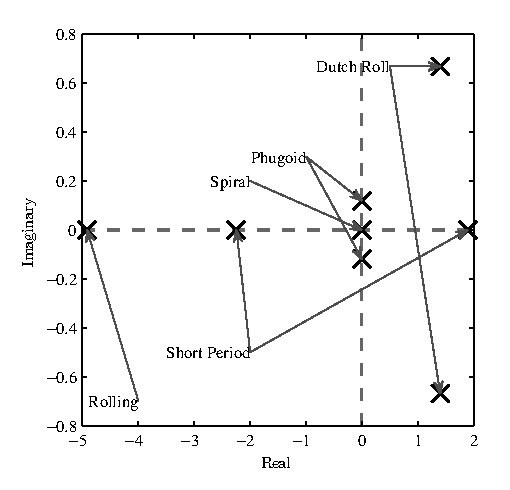
\includegraphics[width=4.0in]{\figurepath/openlooppoles_v2.eps}
  \caption{Open-loop poles of $A$ for $M=6$, $h=80,000$ ft steady, level cruise\label{fig:poleplot}}
\end{figure}

The sensitivity analysis performed above indicates the presence of six flight modes.
These modes are explained below.
\begin{itemize}\itemsep2pt
  \item{\textbf{Short Period} ($\lambda_{1,3}$) \textemdash{} an unstable mode dominated by $\alpha$ and $q$. Relatively fast, purely real poles, with $\lambda_{1,3}\approx\pm2$.}
  \item{\textbf{Rolling} ($\lambda_{2}$) \textemdash{} a stable mode, dominated by $\beta$ and $p$. Fast, real pole at $\lambda_{2}=-4.9$.}
  \item{\textbf{Dutch-Roll} ($\lambda_{4,5}$) \textemdash{} an unstable mode, which is a combination of a rolling, pitching, and yawing motion in flight.}
  \item{\textbf{Phugoid} ($\lambda_{6,7}$) \textemdash{} a neutrally stable phugoid-type mode.}
  \item{\textbf{Velocity} ($\lambda_{8}$) \textemdash{} neutrally stable.}
  \item{\textbf{Spiral} ($\lambda_{9}$) \textemdash{} a slow, but stable mode.}
\end{itemize}
The eigenvalues corresponding to the different modes are shown in the pole plot in Figure~\ref{fig:poleplot}.
The pole corresponding to the velocity mode is dropped, since it has no affect on any of the other longitudinal dynamics.
This stability analysis was repeated at several other flight conditions, and revealed the same basic modes, although the pole locations and stability of some of the modes differed from the flight condition shown here.

This analysis allowed the velocity, longitudinal, and lateral-directional subsystems to be decoupled, and each of these three plant subsystems to be represented as
\begin{equation}
  \label{eqn:plantxp}
  \dot{x}_{p}=A_{p}x_{p}+B_{p}u
\end{equation}
where $x_{p}\in\mathbb{R}^{n_{p}}$, $A_{p}\in\mathbb{R}^{n_{p}\times n_{p}}$, $B_{p}\in\mathbb{R}^{n_{p}\times m}$ and $u\in\mathbb{R}^{m}$.
Note that these sizes will differ for each of the subsystems.

\section{Uncertainties}

A model is only a mathematical representation of a system or process, and so the presence of uncertainty in any plant model is inevitable.
This is particularly true in the case of a hypersonic vehicles, due in part to engine/airframe coupling, complex shock interactions, flexible effects, and unsteady aerodynamics\ \cite{mcruer.hypersonic.1991,schmidt.dynamics.1992,rudd.hypersonic.2010}.
Many of these uncertainties can be represented as parametric uncertainties as shown in (\ref{eqn:linearuncertainties}), and include unknown aerodynamic coefficients and control ineffectiveness, among others.

When building a more conventional vehicle such as a subsonic transport aircraft, much wind tunnel and flight test data is collected, and the aerodynamic coefficients describing the aircraft can in general be determined with a high level of accurately\ \cite{maine.coefficients.1981,morelli.parameters.1997}.
This data is difficult to obtain for a hypersonic vehicle, where wind tunnel testing is more difficult to do.
Additionally an extremely limited amount of hypersonic flight test data has ever been recorded, especially for air-breathing hypersonic vehicles.
Existing analytical techniques often fail to accurately predict the stability derivatives for air-breathing vehicles due to hypersonic flow assumptions which are violated due to the presence of the engine\ \cite{rudd.integrated.2000}.
The use of CFD has become increasingly used to model the aerodynamics of hypersonic vehicles, but there is still much work to be done.

Because of these challenges, uncertainties in the values of the aerodynamic properties, such as given by stability derivatives, of up to several hundred percent are possible in a hypersonic vehicle.
Loss in control effectiveness can occur through damage, as well as for similar reasons as above: the aerodynamic moments generated by a control surface deflection are not great as predicted through modeling.
Center-of-gravity shifts are represented in a similar way as some of the stability derivative uncertainties, having an effect of altering the moments of the vehicle.
The center of gravity uncertainties may be due to fuel burn during flight, or simply errors made when building the aircraft.

\subsubsection*{Control Surface Effectiveness}

The loss of control effectiveness for a hypersonic vehicle was described briefly above.
The loss in control effectiveness could be due to modeling errors, or damage sustained during flight, as depicted in Figure~\ref{fig:flapdamage}.

\begin{figure}[H]
  \begin{center}
    
\includegraphics[width=2.0in]{\figurepath/flap2.eps}
    \caption{Uncertainty in control effectiveness due to control surface damage\label{fig:flapdamage}}
  \end{center}
\end{figure}

\subsubsection*{Center of Gravity Shift}

Conventional aircraft can typically have significant variations in center of location.
These variations are minimized by careful loading of the aircraft, and by placing fuel tanks as close as is practicable to the center of gravity location so as to minimize the CG shift due to fuel burn.
The GHV will not be carrying any auxiliary payload, and it is the goal to have fuel tanks which are as close to the CG as possible.
Even so, uncertainty in the center of gravity location is inevitable and can greatly impact the stability of the vehicle.

\subsubsection*{Pitching Moment Coefficient}

While all of the aerodynamic coefficients will have some uncertainty, it was decided to study uncertainty in the pitching moment coefficient due to its effect on the unstable short period dynamics of the GHV.\@

\subsection{Representation of Uncertainties}\label{sec:repofuncertainties}

It can be shown that the parametric uncertainties considered in this work and described above manifest themselves in the linear system given in Equation (\ref{eqn:plantxp}) as
\begin{equation}
  \label{eqn:xdotpunc}
  \dot{x}_{p}=A_{p\lambda}x_{p}+B_{p\lambda}u
\end{equation}
where
\begin{equation}
  \label{eqn:linearuncertainties}
  A_{p\lambda}=A_{p}+B_{p}\Lambda{W_{p}}^{\top}
  \hspace{0.5in}
  B_{p\lambda}=B_{p}\Lambda
\end{equation}
$\Lambda\in\mathbb{R}^{m\times m}$ and $W_{p}\in\mathbb{R}^{n_{p}\times m}$.
These uncertainties are called ``matched'' uncertainties, as they enter the system dynamics through the control channels\ \cite{lavretskywise.book.2013}.
The adaptive controller that is designed in Section~\ref{sec:adaptivedesign} is carried out so as to accommodate such uncertainties.
Other unmatched uncertainties, such as sensor bias/noise are introduced as well, and the control design must be sufficiently robust to these, as they are not accommodated for explicitly in the synthesis of the controller.
